\setcounter{framenumber}{0}
%37


\begin{frame}
  \titlepage
\end{frame}

\begin{frame}{Learning Goals}
By the end of this lecture, students should be able to:

\begin{itemize}
    \item apply the multiplication rule for counting;
    \item distinguish between sampling with and without replacement;
    \item compute permutations and ordered selections;
    \item compute combinations and unordered selections;
    \item understand the binomial coefficient combinatorially;
    \item recognize and avoid overcounting;
    \item prove combinatorial identities using counting arguments.
\end{itemize}
\end{frame}

\lecturepart{The Multiplication Rule (Product Rule)}

\begin{frame}{The Basic Counting Principle}
\begin{keybox}{Multiplication Rule}
Suppose a procedure consists of two stages.

\begin{itemize}
    \item Stage 1 can be done in $\bf 
    a$ ways;
    \item for each choice in Stage 1, Stage 2 can be done in $\bf b$ ways.
\end{itemize}

Then the entire procedure can be done in

\[
\bf a \times  b
\]

ways.
\end{keybox}

More generally, if a process has stages with
\[
n_1,n_2,\dots,n_k
\]
possible choices respectively, then the total number of outcomes is $n_1n_2\cdots n_k.$

\end{frame}

\begin{frame}{Tree Interpretation}
The multiplication rule can be visualized using a tree.

\vspace{0.3cm}

Suppose:
\begin{itemize}
    \item there are $3$ choices for the first step;
    \item each leads to $2$ choices for the second step.
\end{itemize}

Then, according to the Multiplication Rule, there are $3 \times 2 = 6$ possible outcomes.

\begin{center}
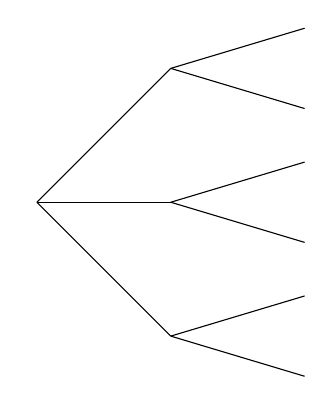
\begin{tikzpicture}[scale=0.85]
\node at (0,0) {};
\foreach \y in {2,0,-2}
{
    \draw (0,0) -- (2,\y);
    \draw (2,\y) -- (4,\y+0.6);
    \draw (2,\y) -- (4,\y-0.6);
}
\end{tikzpicture}
\end{center}
\end{frame}

\begin{frame}{Example: License Plates}
Suppose a license plate consists of $3$ letters,
followed by $4$ digits. Assume repetition is allowed.
\begin{figure}
    \centering
    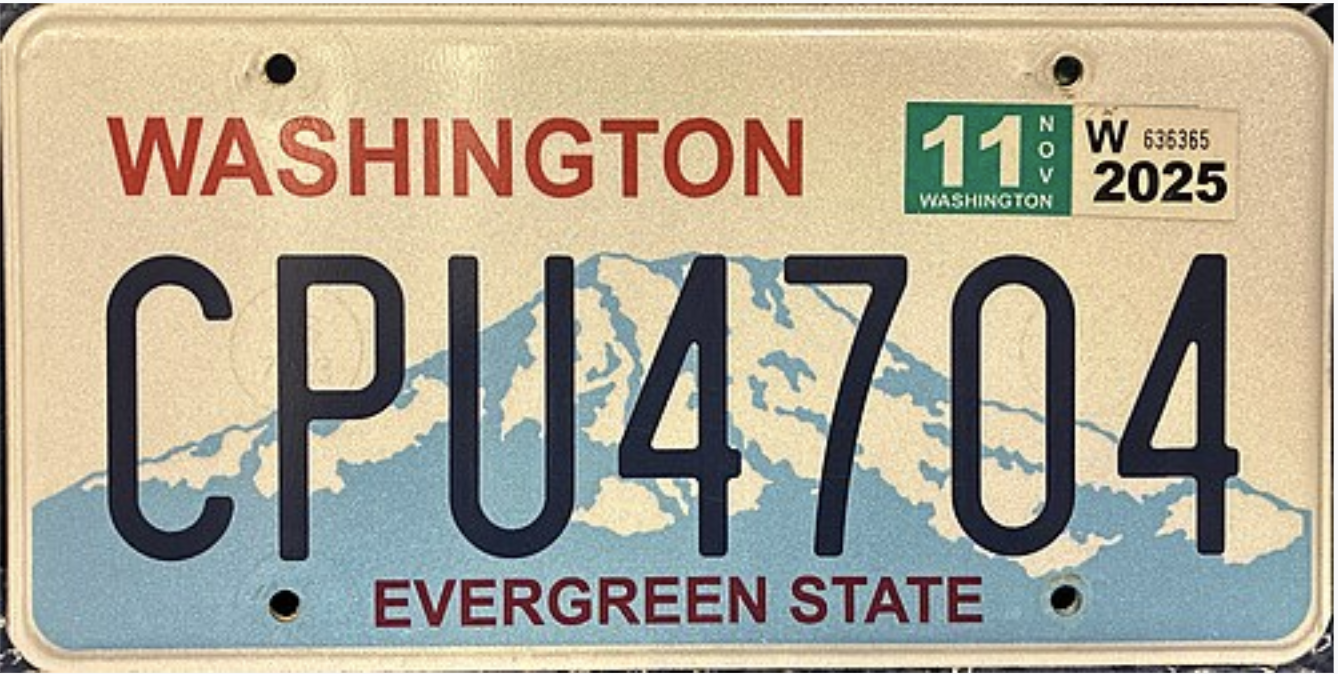
\includegraphics[width=0.25\textwidth]{assets/figures/wa.png}
    \caption{\scriptsize WA license plate. Source: Wikipedia.}
\end{figure}

Choices:
\[
26 \text{ possibilities for each letter},
\]
\[
10 \text{ possibilities for each digit}.
\]

Thus the total number of possible license plates is

\[
(26\times 26 \times 26 ) \times (10 \times 10 \times 10 \times 10) = 26^3 \cdot 10^4 = 175,760,000\ \ (?!)
\]
\end{frame}

\begin{frame}{Example: Binary Strings}
A binary string of length $n$ consists only of $0$'s and $1$'s.

\vspace{0.25cm}

Each position has:
\[
2 \text{ choices}.
\]

Using the multiplication rule:
\[
\underbrace{
\begin{array}{c}
\fbox{$2$}\\[-1mm]
{\text{\scriptsize 0 or 1}}
\end{array}
}_{\text{position }1}
\times
\underbrace{
\begin{array}{c}
\fbox{$2$}\\[-1mm]
{\scriptsize 0 or 1}
\end{array}
}_{\text{position }2}
\times
\cdots
\times
\underbrace{
\begin{array}{c}
\fbox{$2$}\\[-1mm]
{\scriptsize 0 or 1}
\end{array}
}_{\text{position }n}
=
2^n.
\]

Therefore, Number of binary strings of length $n$ is  $2^n$.

Remark: This is also equal to the number of all possible subsets of a set with $n$ elements. (Why?)
\end{frame}

\lecturepart{Sampling With and Without Replacement}





\begin{frame}{Ordered Sampling With Replacement}

Suppose we have a set of size $n$, and we perform $k$ draws with replacement, where $1\leq k \leq n$.

\vspace{0.25cm}

\textbf{With replacement} means:
after each draw, the selected object is returned before the next draw.

\vspace{0.35cm}

Therefore, each draw has exactly $n$ possible choices.

\vspace{0.25cm}

Using the multiplication rule:

\[
\underbrace{
\begin{array}{c}
\fbox{$n$}\\[-1mm]
{\text{\scriptsize choices}}
\end{array}
}_{\text{draw }1}
\times
\underbrace{
\begin{array}{c}
\fbox{$n$}\\[-1mm]
{\text{\scriptsize choices}}
\end{array}
}_{\text{draw }2}
\times
\cdots
\times
\underbrace{
\begin{array}{c}
\fbox{$n$}\\[-1mm]
{\text{\scriptsize choices}}
\end{array}
}_{\text{draw }k}
=
n^k.
\]

\vspace{0.25cm}

Hence, the number of possible ways to draw $k$ ordered items, with replacement, from a set of size $n$, is 

\[
{n^k}.
\]

\end{frame}

\begin{frame}{Example: PIN Codes}
A $4$-digit PIN code uses digits $0$--$9$.

Digits may repeat.

\vspace{0.25cm}

Each position has:
\[
10 \text{ choices}.
\]

Therefore:

\[
10^4 = 10000
\]

possible PINs.
\end{frame}





\begin{frame}{Ordered Sampling Without Replacement}

Now suppose selected objects are \emph{not} returned after each draw.

\vspace{0.25cm}

Then the number of available choices decreases after every selection.

\vspace{0.35cm}

Using the multiplication rule:

\[
\underbrace{
\begin{array}{c}
\fbox{$n$}\\[-1mm]
{\text{\scriptsize choices}}
\end{array}
}_{\text{draw }1}
\times
\underbrace{
\begin{array}{c}
\fbox{$n-1$}\\[-1mm]
{\text{\scriptsize choices}}
\end{array}
}_{\text{draw }2}
\times
\underbrace{
\begin{array}{c}
\fbox{$n-2$}\\[-1mm]
{\text{\scriptsize choices}}
\end{array}
}_{\text{draw }3}
\times
\cdots
\times
\underbrace{
\begin{array}{c}
\fbox{$n-k+1$}\\[-1mm]
{\text{\scriptsize choices}}
\end{array}
}_{\text{draw }k}
\]

\[
= n(n-1)(n-2)\cdots(n-k+1)=\frac{n!}{(n-k)!}.
\]

\vspace{0.25cm}

\begin{keybox}{Important}
Without replacement means that the choices depend on previous selections.
\end{keybox}

\end{frame}













\begin{frame}{Example: Arranging Books}
Suppose $5$ distinct books are arranged on a shelf.

\vspace{0.25cm}

Choices:
\[
5 \text{ choices for the first position},
\]
\[
4 \text{ for the second},
\]
\[
3 \text{ for the third},
\]
etc.

Therefore, the number of arrangements is

\[
5\cdot4\cdot3\cdot2\cdot1 = 5! = 120.
\]

\end{frame}

\lecturepart{Factorials and Permutations}

\begin{frame}{Factorials}
\begin{keybox}{Definition}
For a positive integer $n$,

\[
n! = n(n-1)(n-2)\cdots2\cdot1.
\]

Also define

\[
0! = 1.
\]
\end{keybox}

\vspace{0.25cm}

Examples:
\[
1!=1,
\qquad
2!=2,
\qquad
3!=6,
\qquad
4!=24,
\qquad
5!=120.
\]
\end{frame}

\begin{frame}{Permutations}
A \textbf{permutation} is an ordered arrangement.

\vspace{0.25cm}

The number of ordered ways to choose $k$ objects from $n$ distinct objects is

\[
n(n-1)\cdots(n-k+1).
\]

Using factorial notation:

\[
{
\frac{n!}{(n-k)!}
}
\]

This is denoted by

\[
P(n,k).
\]
So, in summary
$$P(n,k) = \frac{n!}{(n-k)!} = n(n-1)\cdots(n-k+1).$$

\end{frame}

\begin{frame}{Example: Choosing Officers}
Suppose a club has $12$ members.

We choose:
\begin{itemize}
    \item a president,
    \item a vice president,
    \item a secretary.
\end{itemize}

Since positions are different, order matters.

\vspace{0.25cm}

Therefore:

\[
P(12,3) = \frac{12! }{9!}=12\cdot11\cdot10
=
1320.
\]

\end{frame}

\lecturepart{Combinations}

\begin{frame}{When Order Does Not Matter}
Suppose we choose a committee of size $k$ from $n$ people.

\vspace{0.25cm}

Now:
\[
\{A,B,C\}
\]
and
\[
\{B,A,C\}
\]
represent the same committee.

\vspace{0.25cm}

Thus order does \textbf{not} matter.

\vspace{0.25cm}

This requires a different counting formula.
\end{frame}

\begin{frame}{Binomial Coefficients}
\begin{keybox}{Definition}
The number of subsets of size $k$ from a set of size $n$ is

\[
\binom{n}{k}
=
\frac{n!}{k!(n-k)!}.
\]
\end{keybox}

\vspace{0.25cm}

This is read as:
\[
\text{``$n$ choose $k$''}.
\]


Note: $\binom{1}{1} =  \binom{1}{0} = \binom{0}{0} =1 $, can be justified by the formula or combinatorially.
\end{frame}

\begin{frame}{Why Divide by $k!$?}
Suppose we first count ordered selections:

\[
P(n,k) = \frac{n!}{(n-k)!}.
\]

But each unordered subset is counted many times.

\vspace{0.25cm}

For example $\{A,B,C\}$
can appear as:
\[
ABC,\ ACB,\ BAC,\ BCA,\ CAB,\ CBA.
\]
There are 3! = 6  orderings.

Therefore we divide by $k!$:

\[
\binom{n}{k}
=
\frac{n!}{k!(n-k)!} = \frac{P(n,k)}{k!} \Rightarrow  \binom{n}{k} \leq P(n,k).
\]
\end{frame}

\begin{frame}{Example: Poker Hands}
A poker hand consists of $5$ cards from a $52$-card deck.

Order does not matter.

\vspace{0.25cm}

Thus the number of poker hands is

\[
\binom{52}{5}
=
\frac{52!}{5!47!}.
\]

\vspace{0.25cm}

\end{frame}

\begin{frame}{Example: Committees}
How many committees of size $4$ can be formed from $10$ people?

\vspace{0.25cm}

Since order does not matter:

\[
\binom{10}{4}
=
\frac{10!}{4!6!}.
\]

Simplifying:

\[
\binom{10}{4}=210.
\]
\end{frame}

\lecturepart{Properties of Binomial Coefficients}

\begin{frame}{Symmetry Identity}
\begin{keybox}{Identity}
\[
\boxed{
\binom{n}{k}
=
\binom{n}{n-k}
}
\]
\end{keybox}

\vspace{0.25cm}

Reason:

Choosing $k$ elements to include is equivalent to choosing $n-k$ elements to exclude. :)


Algebraic Proof:
\end{frame}


\begin{frame}{Khayyam--Pascal's Identity}
\begin{keybox}{Khayyam-Pascal's Identity}
\[
\boxed{
\binom{n}{k}
=
\binom{n-1}{k}
+
\binom{n-1}{k-1}
}
\]
\end{keybox}
\end{frame}

\begin{frame}{Combinatorial Proof of Khayyam-Pascal's Identity}
Suppose a committee of size $k$ is selected from $n$ people.

Focus on one distinguished person.

Two possibilities:

\begin{enumerate}
    \item The distinguished person is not selected.

    Then choose all $k$ members from the remaining $n-1$ people:
    \[
    \binom{n-1}{k}.
    \]

    \item The distinguished person is selected.

    Then choose the remaining $k-1$ members from the remaining $n-1$ people:
    \[
    \binom{n-1}{k-1}.
    \]
\end{enumerate}

Adding the two cases gives (why addition?)

\[
\binom{n}{k}
=
\binom{n-1}{k}
+
\binom{n-1}{k-1}.
\]
\end{frame}


\begin{frame}{Khayyam--Pascal Triangle: The Main Idea}

The Khayyam--Pascal triangle is a triangular arrangement of numbers.

\vspace{0.25cm}

Each row begins and ends with $1$.

\vspace{0.25cm}

Every interior entry is obtained by adding the two entries directly above it:





\begin{tcolorbox}[
colback=blue!5,
colframe=blue!70!black,
arc=2mm,
boxrule=0.8pt,
left=2mm,
right=2mm,
top=1mm,
bottom=1mm
]
\[
\text{new entry} = \text{upper-left entry} + \text{upper-right entry}\]
\end{tcolorbox}








\[
\begin{array}{ccccccccc}
&&&&1&&&&\\[1mm]
&&&1&&1&&&\\[1mm]
&&1&&2&&1&&\\[1mm]
&1&&3&&3&&1&\\[1mm]
1&&4&&6&&4&&1
\end{array}
\]

\vspace{0.2cm}

{\scriptsize Source: \href{https://en.wikipedia.org/wiki/Pascal\%27s_triangle}{Wikipedia: Pascal's Triangle}.}

\end{frame}


\begin{frame}{Building the Triangle}

Start with $1$ at the top.

\vspace{0.25cm}

Each new number is the sum of the two numbers above it.

\[
\begin{array}{ccccccccc}
&&&&1&&&&\\[2mm]
&&&1&&1&&&\\[2mm]
&&1&&\boxed{1+1}&&1&&\\[2mm]
&1&&\boxed{1+2}&&\boxed{2+1}&&1&\\[2mm]
1&&\boxed{1+3}&&\boxed{3+3}&&\boxed{3+1}&&1
\end{array}
\]


\end{frame}
\begin{frame}{The Formula Inside the Triangle}

\small

\[
\renewcommand{\arraystretch}{1.35}
\begin{array}{ccccccccccccccccc}

\text{row }0
&&&&&&&& \binom{0}{0} &&&&&&&&  \\

\text{row }1
&&&&&&& \binom{1}{0} && \binom{1}{1} &&&&&&&  \\

\text{row }2
&&&&&& \binom{2}{0} && \binom{2}{1} && \binom{2}{2} &&&&&&  \\

\text{row }3
&&&&& \binom{3}{0} && \binom{3}{1} && \binom{3}{2} && \binom{3}{3} &&&&&  \\

&&&&&&&& \vdots &&&&&&&& \\[1mm]

\text{row }n-1
&&
\binom{n-1}{0}
&&
\cdots
&&
{\binom{n-1}{k-1}}
&&
{\binom{n-1}{k}}
&&
\cdots
&&
\binom{n-1}{n-1}
&&&&
\\[2mm]

\text{row }n
&
\binom{n}{0}
&&
\cdots
&&
\binom{n}{k-1}
&&
{\binom{n}{k}}
&&
\binom{n}{k+1}
&&
\cdots
&&
\binom{n}{n}
&&&
\end{array}
\]

\vspace{0.35cm}

Each interior entry is obtained by adding the two entries directly above it:

\[
\boxed{
\binom{n}{k}
=
\binom{n-1}{k-1}
+
\binom{n-1}{k}
}
\]

\vspace{0.15cm}

This identity is known as \textbf{Khayyam-Pascal's Rule}.

\end{frame}



\begin{frame}{Khayyam-Pascal's Rule/Identity}

The rule for building the triangle is





\begin{tcolorbox}[
enhanced,
colback=white,
colframe=blue!70!black,
drop shadow,
arc=2mm,
boxrule=0.8pt
]
\[
\binom{n}{k}
=
\binom{n-1}{k-1}
+
\binom{n-1}{k}
\]
for $1\leq k\leq n-1$.
\end{tcolorbox}









\vspace{0.3cm}

For example,

\[
\binom{4}{2}
=
\binom{3}{1}
+
\binom{3}{2}
=
3+3
=
6.
\]

\vspace{0.25cm}

So every interior entry is obtained by adding the two entries above it.

\end{frame}


\begin{frame}{Connection to Binomial Expansions}

The rows of the triangle give the coefficients in binomial expansions.

\[
(a+b)^0 = 1
\]
\[
(a+b)^1 = a+b
\]
\[
(a+b)^2 = a^2+2ab+b^2
\]
\[
(a+b)^3 = a^3+3a^2b+3ab^2+b^3
\]
\[
(a+b)^4 = a^4+4a^3b+6a^2b^2+4ab^3+b^4
\]

\vspace{0.25cm}

\begin{itemize}
    \item The coefficients are exactly the rows of the Khayyam--Pascal triangle. 

\item Hence, we can show that $(a+b)^n = \sum_{k=0}^n \binom{n}{k} a^k b^{n-k}$ (a very useful identity in Probability theory. 

\item Also proves why $2^n = \sum_{i=0}^n \binom{n}{k}$. 

Hint: 2 = 1 + 1 :)
\end{itemize}

\end{frame}

\lecturepart{Story Proofs and Overcounting}

\begin{frame}{Story Proofs}
A \textbf{story proof} proves an identity by showing that both sides count the same object in different ways.

\vspace{0.25cm}

Advantages:

\begin{itemize}
    \item gives intuition;
    \item explains why identities are true;
    \item often simpler than algebraic proofs.
\end{itemize}
\end{frame}

\begin{frame}{Example Story Proof}
\begin{keybox}{Identity}
\[
\sum_{k=0}^{n}\binom{n}{k}=2^n.
\]
\end{keybox}

\vspace{0.25cm}

Why?

\vspace{0.2cm}

The left-hand side counts subsets of an $n$-element set by grouping according to subset size.

\vspace{0.25cm}

The right-hand side counts subsets directly (see slide 60):

each element is either:
\[
\text{included}
\quad \text{or} \quad
\text{not included}.
\]

Thus there are
\[
2^n
\]
subsets total.
\end{frame}



\begin{frame}{Mini-Exercises}
\begin{enumerate}
    \item How many binary strings of length $8$ are there?

    \item How many $3$-letter strings can be formed from the English alphabet if repetition is allowed?

    \item How many ordered arrangements of $4$ people can be selected from $10$ people?

    \item How many committees of size $3$ can be formed from $8$ people?

\end{enumerate}

\vspace{0.25cm}

\begin{livebox}{Answers}
\[
2^8=256,
\qquad
26^3,
\qquad
\frac{10!}{6!},
\qquad
\binom83=56.
\]
\end{livebox}
\end{frame}
\begin{frame}{Summary}
\begin{itemize}

    \item Number of ordered length-$k$ sequences from $n$ options (repetition allowed):
    \[
    n^k.
    \]

    \item Number of ordered length-$k$ sequences from $n$ distinct objects (no repetition):
    \[
    \frac{n!}{(n-k)!}.
    \]

    \item Number of permutations of $k$ objects chosen from $n$:
    \[
    P(n,k)=\frac{n!}{(n-k)!}.
    \]

    \item Number of combinations of $k$ objects chosen from $n$:
    \[
    \binom{n}{k}
    =
    \frac{n!}{k!(n-k)!}.
    \]

    \item Fundamental identities for binomial coefficients:
    \[
    \binom{n}{k}
    =
    \binom{n}{n-k},
    \]
    and
    \[
    \binom{n}{k}
    =
    \binom{n-1}{k}
    +
    \binom{n-1}{k-1}.
    \]
\end{itemize}

\vspace{0.25cm}

\begin{keybox}{Next lecture}
Axiomatic probability and the addition rule.
\end{keybox}
\end{frame}